\documentclass[tikz,border=10pt]{standalone}
\begin{document}
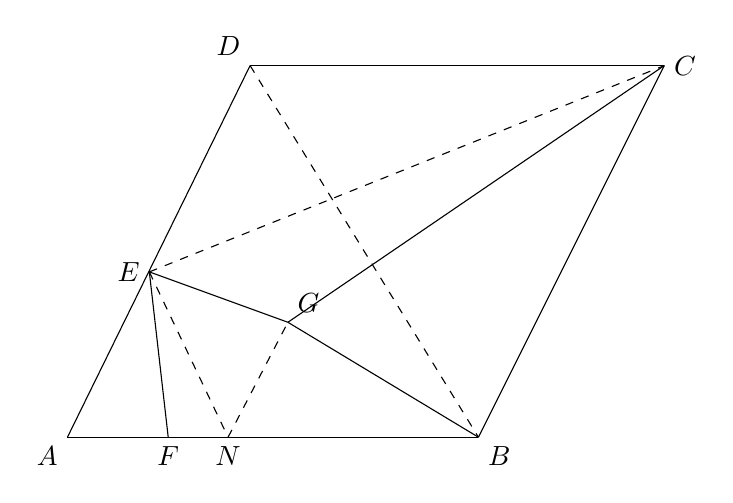
\begin{tikzpicture}[scale=1]
  \coordinate (A) at (1.1,0);
  \coordinate (B) at (6.32,0);
  \coordinate (C) at (8.68,4.72);
  \coordinate (D) at (3.42,4.72);
  \coordinate (E) at (2.14,2.10);
  \coordinate (F) at (2.38,0);
  \coordinate (G) at (3.9,1.46);
  \coordinate (N) at (3.14,0);

  \draw (A) -- (D);
  \draw (D) -- (C);
  \draw (C) -- (B);
  \draw (B) -- (A);
  \draw (E) -- (F);
  \draw (E) -- (G);
  \draw (G) -- (B);
  \draw (C) -- (G);

  \draw[dashed] (E) -- (C);
  \draw[dashed] (D) -- (B);
  \draw[dashed] (E) -- (N);
  \draw[dashed] (N) -- (G);

  \node[above left] at (D) {$D$};
  \node[right] at (C) {$C$};
  \node[below left] at (A) {$A$};
  \node[below right] at (B) {$B$};
  \node[left] at (E) {$E$};
  \node[below] at (F) {$F$};
  \node[above right] at (G) {$G$};
  \node[below] at (N) {$N$};
\end{tikzpicture}
\end{document}
